% !TEX TS-program = pdflatex
% !TEX encoding = UTF-8 Unicode

% Matthew Urffer Master Thesis
% 
% Film Performance
%
\section{Film Performance}

%%%%%%%%%%%%%%%%%%%%%%%%%%%%%%%%%%%%%%%%%%%%%%%%%%%%%%%%%%%%%%%%%%%%%%%%%%%%%%%
%                                                                             %
%                        FILM PERFORMANCE TABLES                              %
%                                                                             %
%%%%%%%%%%%%%%%%%%%%%%%%%%%%%%%%%%%%%%%%%%%%%%%%%%%%%%%%%%%%%%%%%%%%%%%%%%%%%%%
\subsection{Examples}
\begin{frame}{Example Spectra}
\begin{columns}[onlytextwidth]
\begin{column}{0.45\textwidth}
	\begin{figure}
		\centering
		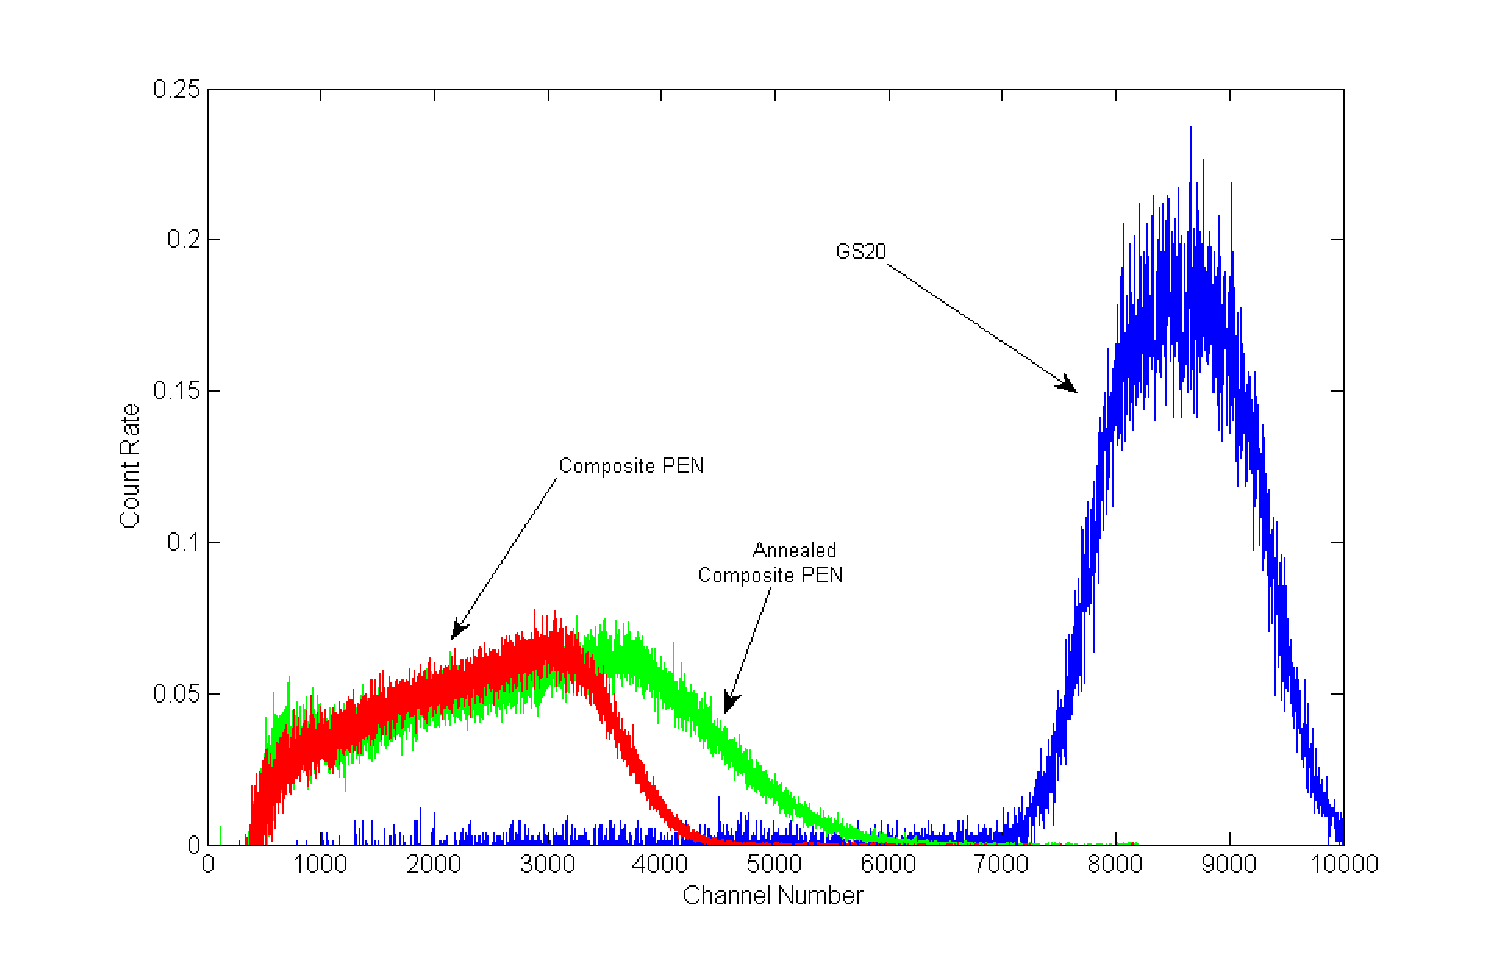
\includegraphics[width=\textwidth]{images/NeutronSpectra.eps}
		\caption{PEN Neutron Spectra}
		\label{fig:PENNeutronSpectra}
	\end{figure}
\end{column}
\begin{column}{0.45\textwidth}
	\begin{figure}
		\centering
		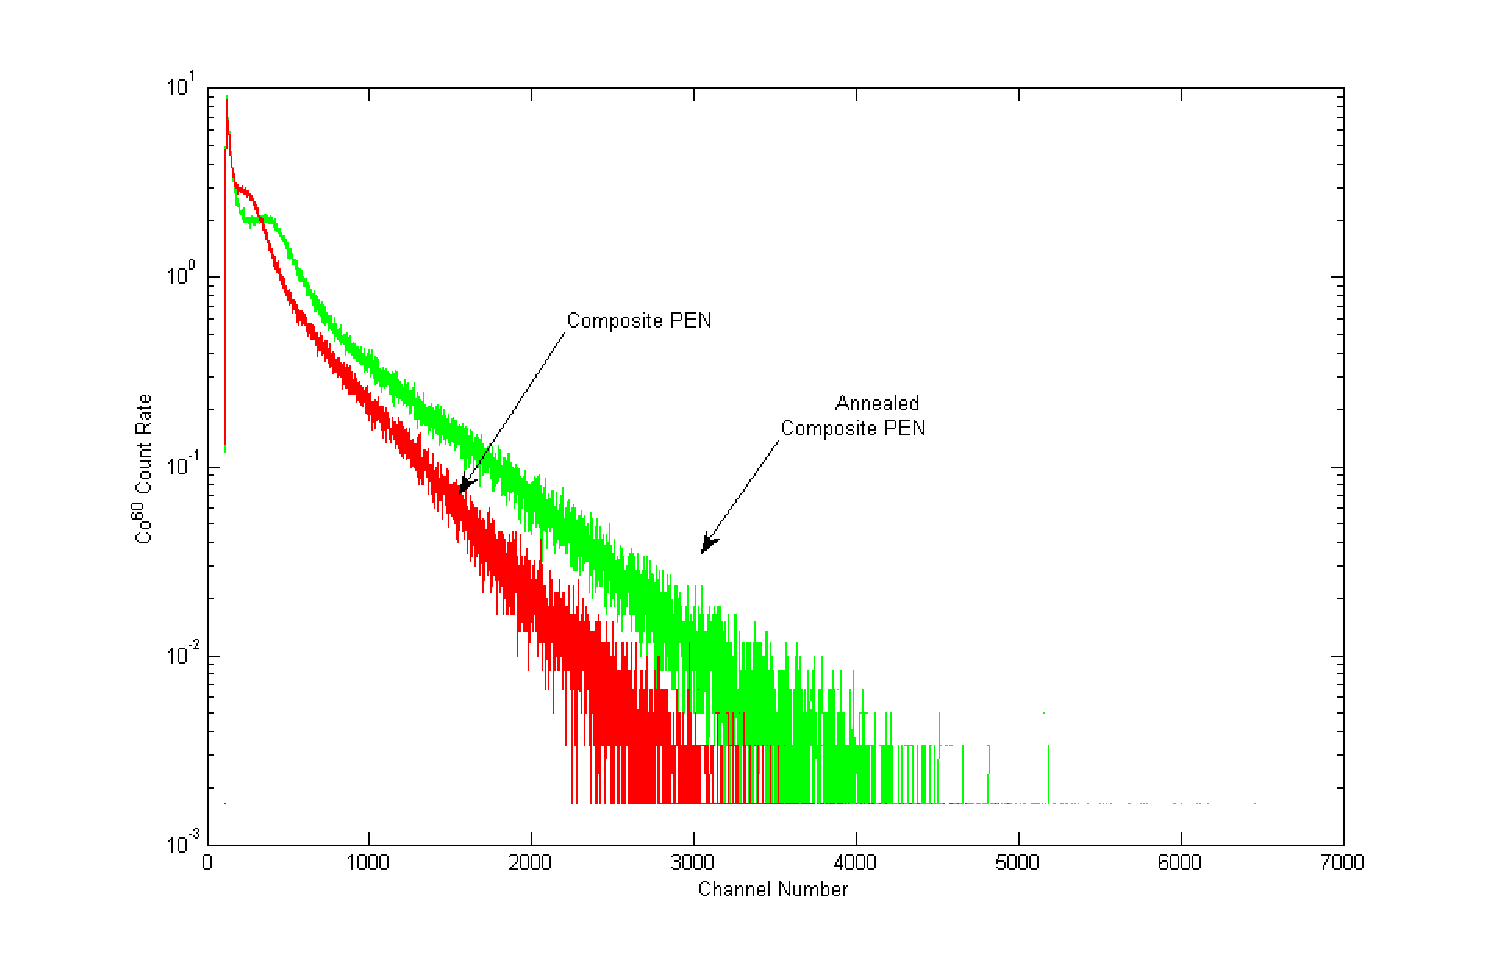
\includegraphics[width=\textwidth]{images/GammaSpectra.eps}
		\caption{PEN Gamma Spectra}
		\label{fig:PENGammaSpectra}
	\end{figure}
\end{column}
\end{columns}
\end{frame}

\subsection{Performance Tables}
%%%%%%%%%%%%%%%%%%%%%%%%%%%%%%%%%%%%%%%%%%%%%%%%%%%%%%%%%%%%%%%%%%%%%%%%%%%%%%%
\begin{frame}{Neutronic and Gamma Efficiency Performance}
	\begin{table}[h]
	\tiny
	\begin{tabular}{m{3cm} >{\centering\arraybackslash}m{2cm} >{\centering\arraybackslash}m{2cm} >{\centering\arraybackslash}m{2cm}}
		 & Absorber Mass (mg) & Total Neutron Count Rate (cps) & Neutron Count Rate above $\epsilon_{int,\gamma} \le 10^{-6}$ (cps) \\
		 \hline
		 \hline
		 PEN 50 \% LiF 1\% ADS156FS (streched) & 9.10 & 53.04 & 11.45 \\
		 \hdashline
		 PEN 70 \% LiF 25\% PPO/POPOPOP 5 \% (158 $\mu$m Annelaed) & 19.6 & 92.4 & 21.2 \\
		 \hdashline
		 PS  LiF 10\% PPO/POPOPOP 5 \% (26 $\mu$m Annelaed) & 1.37 &8.25 & 2.25 \\
		 \hdashline
		 PS  LiF 30\% PPO/POPOPOP 5 \% (50 $\mu$m) & 9.33 & 82.64 & 1.01 \\
		 \hdashline
		 EJ-426 HD2 (LiF in ZnS:Ag) & 105 & 568.3 & 24.56 \\
	\end{tabular}
	\end{table}
\end{frame}

%%%%%%%%%%%%%%%%%%%%%%%%%%%%%%%%%%%%%%%%%%%%%%%%%%%%%%%%%%%%%%%%%%%%%%%%%%%%%%%
\begin{frame}{Light Yield Performance}
	\begin{table}[h]
	\tiny
	\begin{tabular}{m{2cm} >{\centering\arraybackslash}m{1cm} >{\centering\arraybackslash}m{1cm} >{\centering\arraybackslash}m{1cm} >{\centering\arraybackslash}m{1cm} >{\centering\arraybackslash}m{1cm} >{\centering\arraybackslash}m{1cm}}
		 & Alpha Peak (${}^{241}$Am) & Beta Average (${}^{36}$Cl) & $\frac{\alpha}{<\beta>}$ & Photons per Mev (Gamma) & Photons per Mev (Beta) & Photons per Mev (Neturons) \\
		 \hline
		 \hline
		 PEN 50 \% LiF 1\% ADS156FS (streched) & 2,590 & 355 & 0.34 & 500 & 916 & 1,560 \\
		 \hdashline
		 PEN 70 \% LiF 25\% PPO/POPOPOP 5 \% (158 $\mu$m Annelaed) &2,880 & 765 & 0.18 & 1,400 & 1,670 & 2,500 \\
		 \hdashline
		 PS  LiF 10\% PPO/POPOPOP 5 \% (26 $\mu$m Annelaed) & 4,070 & 345 & 0.55 & 1,350 & 1,540 & 1,500\\
		 \hdashline
		 PS  LiF 30\% PPO/POPOPOP 5 \% (50 $\mu$m) & 3,490 & 393 & 0.41 & 1,140 & 1,120 & 1,120 \\
		 \hdashline
		 EJ-426 HD2 (LiF in ZnS:Ag) & & & 19,750 & &26,900 \\
	\end{tabular}
	\end{table}
\end{frame}

